\documentclass[a4paper, titlepage,12pt]{article}
\usepackage[swedish,english]{babel}
\usepackage{listings}
\usepackage{verbatimbox}
\usepackage{xcolor}
\usepackage{pgfplots}
\usepackage{tikz}
\usepackage{amsmath}
\usepackage{float}
\usepackage[backend=biber,citestyle=ieee]{biblatex}
\addbibresource{./literature.bib}
\usetikzlibrary{datavisualization}
\definecolor{codegreen}{rgb}{0,0.6,0}
\definecolor{codepurple}{rgb}{0.5,0,0.5}
\definecolor{backcolor}{rgb}{0.97,0.97,0.97}
\lstdefinestyle{mystyle}{
	commentstyle=\color{codegreen},
	keywordstyle=\color{magenta},
	numberstyle=\color{gray}\ttfamily\footnotesize,
	backgroundcolor=\color{backcolor},
	basicstyle=\ttfamily\footnotesize,
	stringstyle=\color{codepurple},
	numbers=left,
	tabsize=4
}
\lstset{style=mystyle}


\title{Computer Vision\\Assignment 3 \& 4}
\author{Adam Temmel (adte1700)}
\date{\today}

\begin{document}
\maketitle

\section*{Assignment 3}
	\subsubsection*{Mark the following points in a graph. Draw the Hough space for the points (using $\rho$ and $\theta$). In the Hough space, identify the crossing of the graphs (or the ”best possible solution”). Draw the line corresponding to the best solution in the graph.}

	I constructed the following plots (using the $\rho = x cos(\theta) + y sin(\theta)$ formula):

	\begin{figure}[h!]
		\begin{center}
		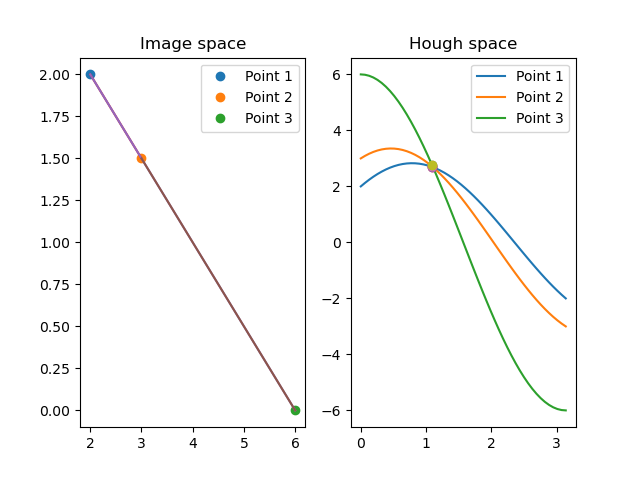
\includegraphics[scale=0.8]{./pts_1.png}
			\caption{Hough space generated from the points (2, 2), (3, 1.5), (6, 0)}
		\end{center}
	\end{figure}

	A line has been drawn between the points which crossing each other.
	\newpage

	\begin{figure}[h!]
		\begin{center}
		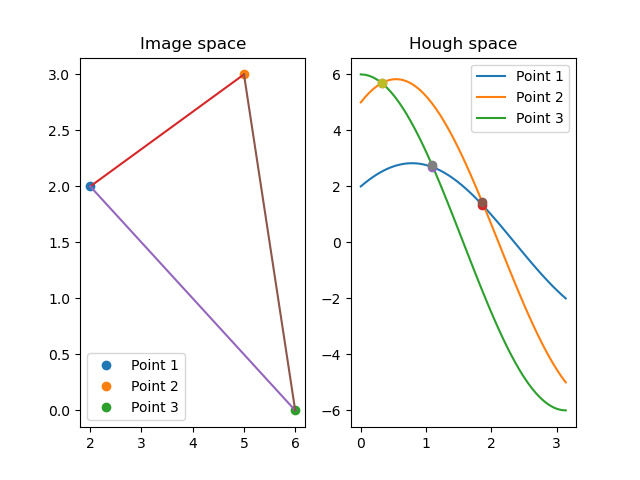
\includegraphics[scale=0.8]{./pts_2.png}
			\caption{Hough space generated from the points (2, 2), (5, 3), (6, 0)}
		\end{center}
	\end{figure}

	Here, several crossings appeared, but only once per point combination. As such, I plotted all of the crossings, as none of the available crossings seemed better or worse than the others. This might not be the way to go about things when you use this to solve a ''real'' problem, but I chose to plot all available data for the sake of completeness.

	\begin{figure}[H]
		\begin{center}
		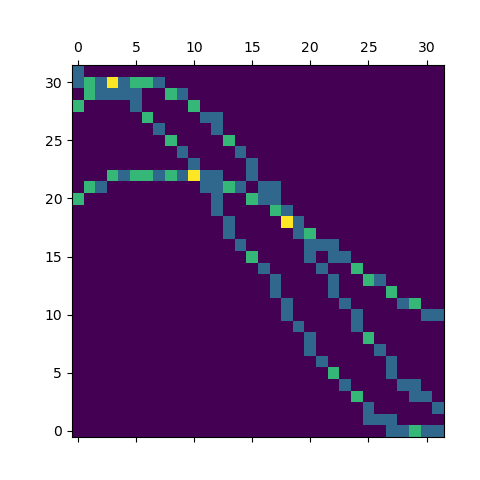
\includegraphics[scale=0.8]{./voting.png}
			\caption{Visualisation of the voting results within the hough space created from the points (2, 2), (5, 3), (6, 0)}
		\end{center}
	\end{figure}

	\subsubsection*{Find out more about the feature descriptors mentioned in the lecture 
by looking into the book, online lectures and the Internet.  Which 
descriptor would you use when in a implementation for Augmented 
Reality? (Hint: There is no correct answer, just good arguments!)}

% sift, surf, brief, orb
	I found a paper which compared some of the feature descriptors mentioned purely in terms of accuracy\cite{feat-comp}. It describes SIFT as being very robust, with the drawback of requiring more computational time when compared to other algorithms. SURF is also presented as a robust algorithm, while being slightly faster than SIFT. BRIEF, while not being scale/orientation invariant requires a lot less processing power than SIFT/SURF. Lastly, ORB is described as being around twice as fast as SIFT, with the drawback of not being scale invariant. As augmented reality in many cases involve the need for real-time computing, computation speed may very well be of interest for this particular field. As such, my answer would be to prefer ORB unless the potential accuracy drop between ORB and its competitors is considered to great, in which SIFT or SURF might be preferable.

	\subsubsection*{Take two picture with your mobile phone, where the images partly 
covers the same scene. Make sure the scene is fairly simple, but 
contains ''flat region''”, “edges” and “corners”}

	\subsubsection*{Implement a feature detector and apply it on the images. Choose among Harris operator, max ($\lambda-$), harmonic mean, Triggs, etc. Remember to smooth the image. E.g. use a ''derivative of Gaussian'' filter.}

	\begin{figure}[h!]
		\begin{center}
		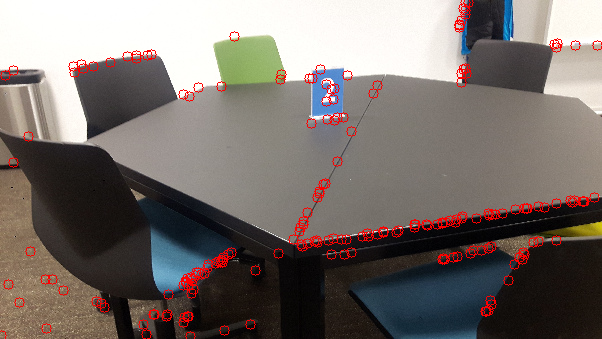
\includegraphics[scale=0.3]{./harris_out_1.png}
		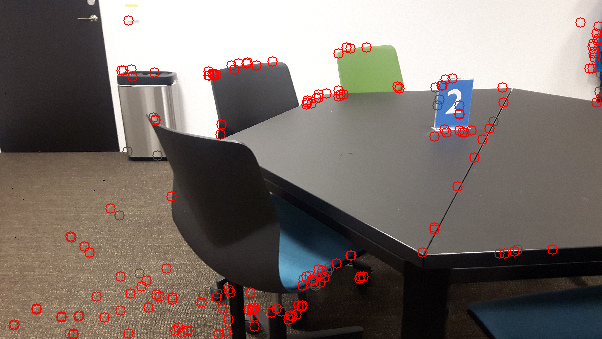
\includegraphics[scale=0.3]{./harris_out_2.png}
			\caption{Feature points extracted from running my own feature detector (Harris) on two similar images}
		\end{center}
	\end{figure}

	\begin{figure}[H]
		\begin{center}
	\begin{lstlisting}[language=Python]
#!/usr/bin/env python

import numpy as np
import cv2

path = './to_detect_2.jpg'	# file to work with
img = cv2.imread(path, 0)	# read as greyscale

# sobel kernels
gx_kernel = np.array([
    [1, 0, -1],
    [2, 0, -2],
    [1, 0, -1],
])

gy_kernel = np.array([
    [ 1,  2,  1],
    [ 0,  0,  0],
    [-1, -2, -1],
])

# blur
blur_img = cv2.GaussianBlur(img, (5,5), 3)
# perform sobel and build tensor components
gx = cv2.filter2D(blur_img, -1, gx_kernel)
gy = cv2.filter2D(blur_img, -1, gy_kernel)
gxy = gx * gy
gx2 = gx ** 2
gy2 = gy ** 2

# See also:
# https://en.wikipedia.org/wiki/Harris_corner_detector
k = 0.06
h, w = img.shape
result = np.array([[0.0] * w for _ in range(h)], float)
for y in range(h):
    for x in range(w):
		# structure tensor, see end of chapter 'Development'
        mat = np.array([
            [gx2[y][x], gxy[y][x]],
            [gxy[y][x], gy2[y][x]],
        ], dtype=float)
		# response calculation, see chapter 
		# 'Response Calculation'
        tr = mat[0,0] + mat[1,1]
        det = mat[0,0] * mat[1,1] - mat[1,0]*mat[0,1]
        result[y][x] = det - (k * (tr * tr))

	\end{lstlisting}
	\caption{First half of implementation of Harris corner detector}
	\end{center}
	\end{figure}

	\begin{figure}[H]
		\begin{center}
	\begin{lstlisting}[language=Python]
# mark points of interest
color_img = cv2.imread(path)
threshold = 24500
for y in range(h):
    for x in range(w):
        if result[y][x] > threshold:
            cv2.circle(color_img, (x, y), 5, (0, 0, 255), 1)
cv2.imwrite("harris_out.png", color_img)
	\end{lstlisting}
			\caption{Second half of implementation of Harris corner detector}
	\end{center}
	\end{figure}

	The Harris corner detector I implemented can be summarized into the following steps:

	\begin{enumerate}
		\item Read a greyscale version of the image you wish to process.
		\item Blur the image.
		\item Apply a Sobel kernel to the blurred image (for both the X and Y directions).
		\item Calculate the structure tensor components.
		\item Apply the response calculation for each pixel within the Sobeled image, resulting in a new matrix with the same dimensions as the image.
		\item For each pixel in the new image, compare its value to a given threshold, if the value is greater than the threshold, this pixel is regarded as a feature point.
	\end{enumerate}

	\subsubsection*{Find an implementation of your favourite feature detector/descriptor (SIFT, ORB, etc.), and apply it on your images. Do you get the same feature points as for your implementation?}

	\begin{figure}[h!]
		\begin{center}
		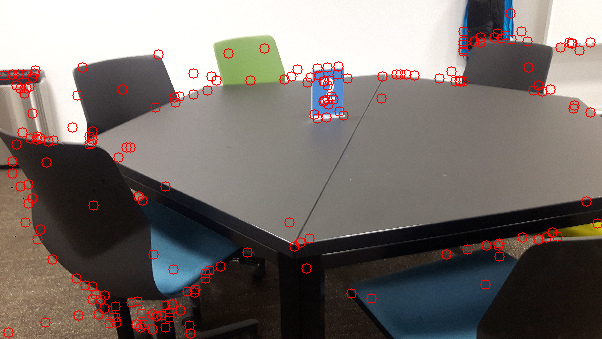
\includegraphics[scale=0.3]{./sift_out_1.png}
		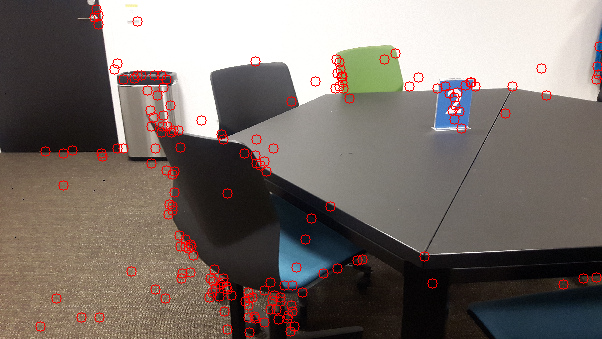
\includegraphics[scale=0.3]{./sift_out_2.png}
			\caption{Feature points extracted from running OpenCV's implementation of the SIFT feature detector on two similar images}
		\end{center}
	\end{figure}

	Although the differences between my implementation of the Harris feature detector and OpenCV's SIFT feature detector were not as many as originally anticipated, my feature detector still introduced an amount of discrepancies large enough for the SIFT feature detector results to be interpreted as better. In particular, the edges of the table were interpreted as corners in my implementation, whereas SIFT is doing a much better job at \textit{only} identifying corners.

	\section*{Assignment 4}

	\subsubsection*{A rectangle is defined by its corners (0,0), (0,3), (5,3), and (5,0).}

	\subsubsection*{Write the similarity transform matrix for the rectangle to move 3 point horizontally, -2 points vertically, turning 15 degrees clockwise.}

	\begin{figure}[H]
	\caption{First half of calculating the total point transform}
	\begin{center}
	\begin{lstlisting}[language=Python]
	#!/usr/bin/env python
import math
import matplotlib.pyplot as plt

corners = [[0, 0, 1], [0, 3, 1], [5, 3, 1], [5, 0, 1]]

# translation matrix
translate = [
    [1, 0,  3],
    [0, 1, -2],
    [0, 0,  1],
]
# rotation matrix
angle = -15
s = math.sin(angle * (math.pi / 180))
c = math.cos(angle * (math.pi / 180))
rotate = [
    [ c, -s, 0],
    [ s,  c, 0],
    [ 0,  0, 1],
]
	\end{lstlisting}
	\caption{First half of calculating the total point transform}
	\label{trans-1}
	\end{center}
	\end{figure}

	\begin{figure}[H]
	\begin{center}
	\begin{lstlisting}[language=Python]
def mat_mul_mat(lhs, rhs):
    m, n, o = len(lhs), len(rhs[0]), len(rhs)
    res = [[0] * n for _ in range(m)]
    for i in range(m):
        for j in range(n):
            for k in range(o):
                res[i][j] += rhs[i][k] * lhs[k][j]
    return res

def mat_mul_vec(lhs, rhs):
    m, n = len(lhs), len(rhs)
    res = [0] * n
    for i in range(m):
        for j in range(n):
            res[i] += lhs[i][j] * rhs[j]
    return res

# total transform
transform = mat_mul_mat(translate, rotate)

# calculate new corners
new_corners = [mat_mul_vec(transform, vec) for vec in corners]

# plot
x1 = [corner[0] for corner in corners]
y1 = [corner[1] for corner in corners]
x2 = [corner[0] for corner in new_corners]
y2 = [corner[1] for corner in new_corners]
plt.xlim([-10, 10])
plt.ylim([-10, 10])
plt.plot(x1, y1, 'o')
plt.plot(x2, y2, 'o')
plt.show()
	\end{lstlisting}
	\caption{Second half of calculating the total point transform}
	\label{trans-2}
	\end{center}
	\end{figure}

	\begin{figure}[H]
		\begin{center}
		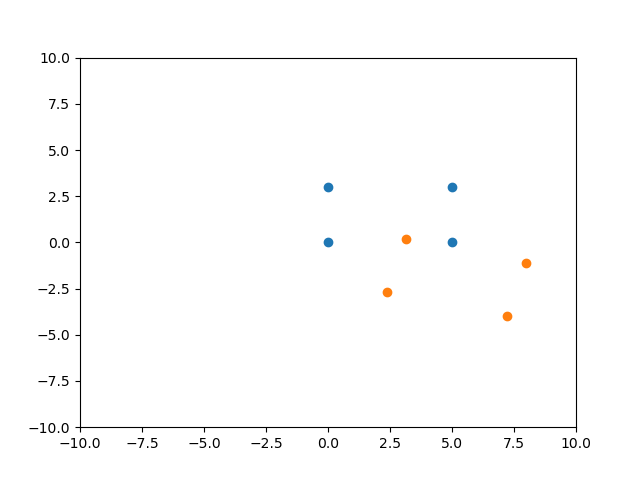
\includegraphics[scale=0.8]{./transform1.png}
			\caption{The resulting plot of the code in figure~\ref{trans-1} and figure~\ref{trans-2}.}
		\end{center}
	\end{figure}

	\subsubsection*{The rectangle is transformed to have it corners at (1,1), (3,3), (6,3), and (5,2). Compute the transformation matrix. You may use Matlab (or similar) to compute the solution}
	\begin{figure}[H]
		\begin{center}
			\begin{lstlisting}[language=Python]
#!/usr/bin/env python
import numpy as np

corners = [[0, 0, 1], [0, 3, 1], [5, 3, 1], [5, 0, 1]]
corners_new = [[1, 1, 1], [3, 3, 1], [6, 3, 1], [5, 2, 1]]

def build_homo(p, q):
    assert(len(p) == len(q))
    assert(len(p[0]) == len(q[0]))
    n = len(p)
    m = len(p[0])
    res = [[0] * (m + 1) * 2 for _ in range(n * 2)]
    for i in range(n):
        v1, v2 = p[i], q[i]
        for j in range(m):
            res[i * 2][j] = v1[j]
            res[i * 2][j + m] = 0
            res[(i * 2) + 1][j + m] = v1[j]
            res[(i * 2) + 1][j] = 0

        res[i * 2][m * 2 + 0] = -v2[0] * v1[0]
        res[i * 2][m * 2 + 1] = -v2[0] * v1[1]

        res[(i * 2) + 1][m * 2 + 0] = -v2[1] * v1[0]
        res[(i * 2) + 1][m * 2 + 1] = -v2[1] * v1[1]

    return res

homo = build_homo(corners, corners_new)
_, _, v = np.linalg.svd(np.array(homo))
h = list(v[-1])
h.append(1)	# append a single 1 to the bottom right corner
h = np.array(h)
print(h.reshape(3, 3))
			\end{lstlisting}
			\caption{Code for calculating the transformation matrix between the corners}
		\end{center}
	\end{figure}

	\begin{figure}[H]
		\begin{center}
			\begin{lstlisting}
$ ./2dtransformations2.py
[[ 0.78820675 -0.32015553  0.02336885]
 [ 0.40298246 -0.16184404 -0.22825153]
 [ 0.15866714 -0.09910638  1.        ]]
			\end{lstlisting}
		\end{center}
	\end{figure}


	\subsubsection*{Check Middlebury web site and find out the principles of some of the best performing stereo algorithms. Write a short description of the one you want to use, and motivate your choice}

	\begin{figure}[H]
		\begin{center}
			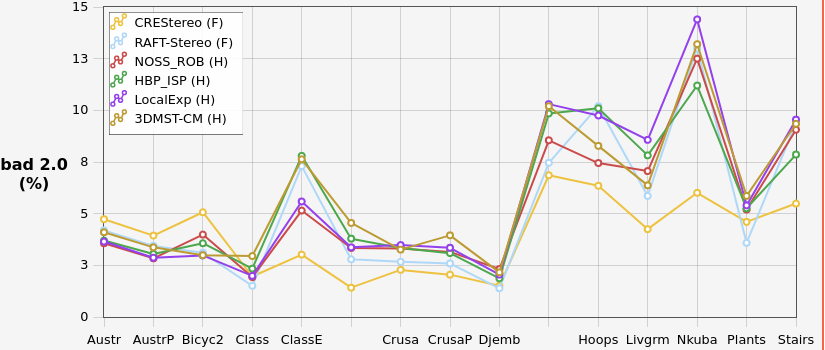
\includegraphics[scale=0.5]{./stereo_stats.png}
			\caption{Graph describing the error rate occured when different stereo algorithms were pitted against eachother.}
		\end{center}
	\end{figure}

	From the list of stereo algorithms presented over at middlebury, one proved to be performing a little bit better than the others in terms of least error rate. This algorithm was named CREStereo, and was submitted by an anonymous user on the 10th of November, 2021. Although no details regarding the algorithm was presented on the site, it is briefly presented as a ''cascaded recurrent network with adaptive correlation''\cite{crestereo}. A cascade-correlation based neural network begins with a network comprised of a very few amount of nodes, instead opting to introduce new nodes to the network iteratively, which in turn entirely avoids the problem of backpropagation.\cite{cascade-correlation}

	\subsubsection*{Take two rectified images from Middlebury’s web page (or use your own rectified images.) Write a short program that performs the plane sweep algorithm. Try out two of the metrics given in Ex 12.4}

	\begin{figure}[H]
		\begin{center}
			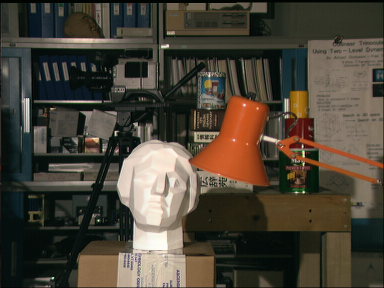
\includegraphics[scale=0.5]{./scene1.row3.col3.png}
			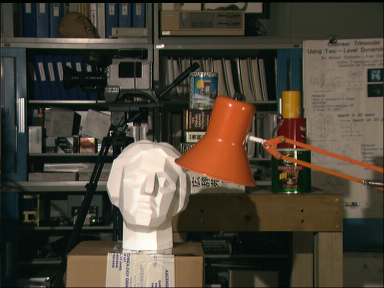
\includegraphics[scale=0.5]{./scene1.row3.col4.png}
			\caption{Two rectified images, courtesy of Middlebury's web page}
		\end{center}
	\end{figure}

	\begin{figure}[H]
		\begin{center}
			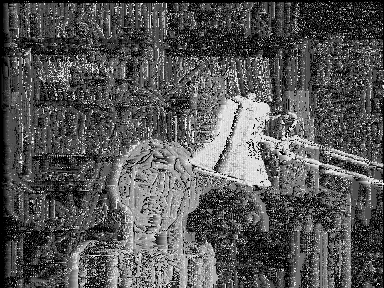
\includegraphics[scale=0.5]{./out_sq_err.png}
			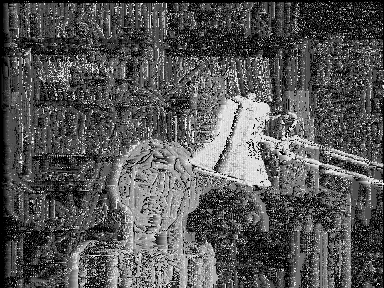
\includegraphics[scale=0.5]{./out_abs_err.png}
			\caption{The output of the plane sweep algorithm, using the squared error for the left image and absolute error for the right image.}
		\end{center}
	\end{figure}

	\begin{figure}[H]
		\begin{center}
			\begin{lstlisting}[language=Python]
#!/usr/bin/env python
import numpy as np
import cv2

left_img = cv2.imread('./scene1.row3.col3.ppm', 0)
right_img = cv2.imread('./scene1.row3.col4.ppm', 0)

def plane_sweep(left_img, right_img, eval_method):
    out_img = np.array([[np.uint8(0)] * len(i) for i in left_img])
    h_img, w_img = left_img.shape
	# for each pixel
    for y_in in range(h_img):
        for x_in in range(w_img):
            min_value = np.Infinity
            suitable_disp = 0
            max_disparity = 16
			# walk to the right 
            for disparity in range(min(max_disparity, x_in + 1)):
				# evaluate the difference between the 
				# images at this location
                result = eval_method(float(left_img[y_in, x_in]) 
					- float(right_img[y_in, x_in - disparity]))
				# if the difference is the lowest
				# difference found so far
                if result < min_value:
					# save it
                    min_value = result
                    suitable_disp = disparity
			# write the lowest difference to the result image
            out_img[y_in, x_in] = ((suitable_disp) 
				/ max_disparity) * 255
    return out_img

img_out_sq_err = plane_sweep(left_img, right_img, lambda x: x ** 2)
img_out_abs_err = plane_sweep(left_img, right_img, lambda x: abs(x))

cv2.imwrite("out_sq_err.png", img_out_sq_err)
cv2.imwrite("out_abs_err.png", img_out_abs_err)
			\end{lstlisting}
			\caption{Code describing an implementation of the plane-sweep algorithm.}
		\end{center}
	\end{figure}

	\subsubsection*{Re-use the images from last week, or take the two new images with your mobile phone; try to keep the camera central point at one position. Identify a number of feature points with your previous code, SIFT or any other feature point detector. Select a subset of these. (You can use RANSAC if you want). Now the actual work: Compute the homography from one image to the other (or to a new image plane) using the SVD-algorithm. Warp (project) the pixels into that plane. (Which warping method shall you use?) Done!}

	\begin{figure}[H]
		\begin{center}
			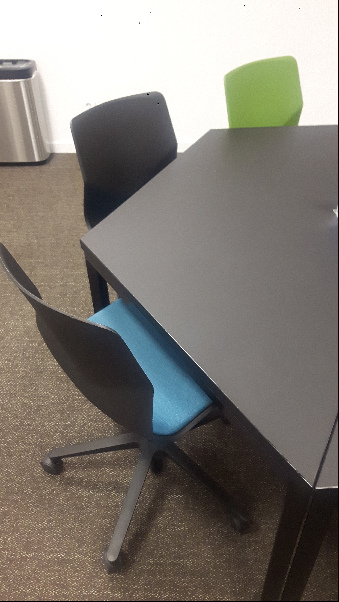
\includegraphics[scale=0.5]{./to_detect_2_1.jpg}
			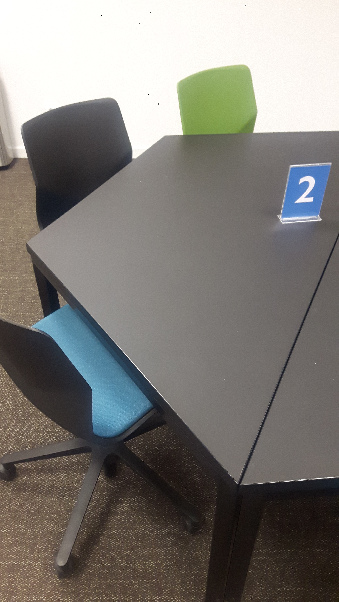
\includegraphics[scale=0.5]{./to_detect_2_2.jpg}
			\caption{The images meant to be stitched together}
		\end{center}
	\end{figure}

	\begin{figure}[H]
		\begin{lstlisting}[language=Python]
#!/usr/bin/env python
import numpy as np
import random
import cv2

def ransac(points_left, points_right, desc_left, desc_right):
	# number of tries
    n = 10000
    best_points = 0
    best_homo = None
    max_len = min(len(points_left), len(points_right))

	# find similiar points in the left and right image
    bf = cv2.BFMatcher()
    matches = bf.match(desc_left, desc_right)
    mp1 = [points_left[m.queryIdx].pt for m in matches]
    mp2 = [points_right[m.trainIdx].pt for m in matches]

    for _ in range(n):
		# take 4 random points
        l = [random.randint(0, max_len - 1) for _ in range(4)]
        p = np.array([mp1[i] for i in l])
        q = np.array([mp2[i] for i in l])

		# try building a homography
        potential_homo, _ = cv2.findHomography(p, q)
        if np.array_equal(potential_homo, None):
            continue # building a homography can fail
		# warp all points
        points_transformed = [potential_homo 
			@ (point[0], point[1], 1) for point in mp1]
        good_points = 0
        for i in range(len(mp1)):
            p_i = points_transformed[i][:2]
            q_i = mp2[i]
            diff = np.linalg.norm(p_i - q_i)
			# evaluate the difference
            if diff < 10:	# if below a threshold
                good_points += 1 # good!
            if best_points < good_points:
                best_points = good_points
                best_homo = potential_homo
    return best_homo # return the best homography found
		\end{lstlisting}
		\caption{Part 1 of the image stitching algorithm}
	\end{figure}
	\begin{figure}[H]
		\begin{lstlisting}[language=Python]

# read in images
path_left = './to_detect_2_1.jpg'
path_right = './to_detect_2_2.jpg'

img_left = cv2.imread(path_left)
img_right = cv2.imread(path_right)

# find feature points
sift = cv2.SIFT_create()
points_left, desc_left = sift.detectAndCompute(img_left, None)
points_right, desc_right = sift.detectAndCompute(img_right, None)

# create a suitable homography using RANSAC
homo = ransac(points_left, points_right, desc_left, desc_right)

# H = homography, l = left image, r = right image
# H * l = r => H^-1 * r = l

# take the inverse of the homography and warp the right
# image into the perspective of the left image
warped = cv2.warpPerspective(img_right, np.linalg.inv(homo), 
		(img_right.shape[1] * 2, img_right.shape[0]))
# splat the left image on top
warped[:img_left.shape[0], :img_left.shape[1]] = img_left

# all done!
cv2.imwrite("stitched.jpg", warped)
		\end{lstlisting}
		\caption{Part 2 of the image stitching algorithm}
	\end{figure}
	\newpage
	\printbibliography
\end{document}
